\subsection{Tableaux Calculus}

Our goal is to produce a model if we can. If we are not able to produce
a model, we want to give an argument, a proof, why this is not possible.
Consider for example the relation \emph{Eat} interpreted as
\[
aEatb \iff \text{a eats b}.
\]
Say we have the following requirement for a pizza: It should be vegetarian
and with salami. This is surely not satisfiable. We want a proof theory
that gives us the same result.

Formally, we use the \emph{Tableaux Calculus} as defined in \cite{gore07}. In the
following $A, B$ usually stand for atoms, while $C,D$ denote concepts. Suppose
we have a set of global assumptions $\Gamma$ and a set of givens $X$. We define
a set of rules, consisting of an `upper' side with the givens, and a `lower' side
with the consequences $Y_i$ as in
\[
(\text{rule}) \, \Gamma: \frac{X}{Y_1 | \dots | Y_k}.
\]
The `denominator' can be seen as the result of a reasoning progress that goes downwards,
i.e. if $X$ is satisfiable, then one of the $Y_i$ is also satisfiable. We define the
following rules:
\[
(\bot) \, \Gamma: \frac{X; A; \lnot A}{\bot}, \quad
(\sqcap) \, \Gamma: \frac{X; C \sqcap D}{X; C; D}, \quad
(\sqcup) \, \Gamma: \frac{X; C \sqcup D}{X; C | X; D},
\]
\[
(\exists R) \, \Gamma: \frac{X; \exists R. C}{\{D | \forall R.D \in X\};  C ; \Gamma}.
\]
Intuitively this means, we can derive falsity from a contradiction ($\bot$), we derive
$C$ and $D$ from knowing that both are true ($\sqcap$), we can derive either $C$ or $D$
from knowing that one of them is true ($\sqcup$). The last rule is a bit more complicated, it
means that whenever we know that there is an $R$-successor that satisfies C, it must
also satisfy $\Gamma$ (because that's true everywhere) and all the things that have
to be true at an $R$-successor, i.e. $\{D | \forall R.D \in X\}$.

Starting with a root with $X$ and $\Gamma$ this gives a tree structure, called a tableaux.
We call a branch closed if the last child is $\bot$ and a tableaux closed if all the
branches are closed. Otherwise, we call the tableaux open. Given a set of global
assumptions $\Gamma$, a set of concepts $X$ is unsatisfiable if and only if there
is a closed tableaux from $\Gamma; X$. We call this a proof. This proof calculus
is sound and complete with respect to $\mathcal{ALC}$. (See e.g. \cite{gore07} for a
proof.)

We can now make a formal argument for the example above. Say we have no global
assumptions, and the two statements $Vegetarian$ and
$\lnot Vegetarian$. We get the simple proof
\[
(\bot) \frac{Vegetarian; \lnot Vegetarian}{\bot}.
\]

We now have the theoretical means to say whether a certain concept is satisfiable
or not. Our program will automate this for us.

\subsection{Description of Main Components}

The program accepts a set of concepts and general assumptions. It then produces
either a model -- demonstrating that the givens are satisfiable -- or a proof
showing unsatisfiablity. The user can choose to get the output in text-format or
a graphical version, or have it just checked for correctness.
The program makes use of the theory presented above to say whether a given concept
is satisfiable or not (assuming some global knowledge). To make sure this is correct
(and convince skeptical users) the program will not just say whether the givens
are satisfiable or not, it will provide the user with either a model or a proof.
The main components are illustrated in Figure~\ref{components}. A \emph{parser} translates
the user input into an internal language that is processed by the
\emph{proof/model searcher}.
In case a model is found, we say it is satisfiable and provide a model that can be
checked by the \emph{model checker}. Otherwise we give a proof that can be checked
by the \emph{proof checker}.

\begin{figure}
  \caption{The main components of the program.}
  \begin{center}
    \includegraphics[scale=0.4]{design.jpeg}
  \end{center}
  \label{components}
\end{figure}

\paragraph{Parser.}

The purpose of the parser is to read the input from the user
and transform it into a format that can be used by the rest of the program. We have
written three different lexers that interpret
\begin{itemize}
\item the user input from the command line (lexerI),
\item modal formulas from the TANCS 2000 Problems\footnote{\url{http://www.cs.man.ac.uk/~schmidt/mspass/problems.html}.} (lexerB1),
\item modal formulas from the logics work bench\footnote{\url{http://iamwww.unibe.ch/~lwb/benchmarks/benchmarks.html}.} (lexerB2).
\end{itemize} 
The actual parser is automatically generated from a grammar we specified.

\paragraph{Proof/Model Searcher.} 

The proof/model searcher receives the knowledgebase and a set of concepts and returns
either a proof or a model. The implementation is similar to the one described in
\cite{gore07}, but additionally a proof and a model are simultaneously build, maintained,
and eventually one of them returned. It consists of the following components:
\begin{itemize}
\item \emph{findProofOrModel}: This is the `entrance' function that maintains
a cache and looks up the current set of concepts. If it is found, it returns the
found result. Otherwise, and certainly in the beginning, the function
\emph{findProofOrModel'} is called. This function expects the concepts to be in
a certain order, so this order is always maintained (using \emph{conceptSort}).

\item \emph{findProofOrModel'}: This function has a case for every possible concept. If no
contradiction is found and it is not done yet, it creates both a model and a proof
after recursively calling \emph{findProofOrModel} on the remainder. For the more
complicated
exists case it calls the function \emph{foldExists}. When it is done, and there was no
contradiction, it calls \emph{constructAtomicModel} to create a model.

\item \emph{foldExists}: It deals with all the exists formulas, by going through them
one by one and generating a proof or model with \emph{applyExists}
for each of them. If a proof is found for one of
the successors, this proof is immediately returned. If all the exists formulas
supplied models, they are joined using \emph{joinModels} and returned. Because
the function has to keep track of the individuals used in each model, we decided
to choose a `fold' approach with caching in favor of parallelism.
\end{itemize}
The result is either a proof or a model, which can be checked with the proof and
model checkers.


\paragraph{Proof Checker.}

The main purpose of the proof checker component of the program is to ensure the proof produced by the proof construction component is: correctly formed, independent of the implementation of the proof search; and proves unsatisfiability given the initial set of formulas and global assumptions. However, the proof checker will check any proof structure passed to it, including proofs that may be given by the user rather than produced by the proof construction component of our program.

 The proof checker is called by the function checkProof with the actual proof tree to check and the global assumptions that the proof was constructed against as expected inputs. The expected output of the proof checker is a tuple consisting of a String and a Boolean. The Boolean has the value True when each step in the proof applies a proof rule correctly in the tableau calculus described in the Background section; and shows unsatisfiability by closing with a contradiction or falsity in all branches of the proof. Otherwise, the Boolean returned has the value False and the String is a message detailing why the proof tree is incorrect or does not show unsatisfiability. Hence the string is empty if the proof tree is correct.

 The proof checker is made up of the following components:

\begin{itemize}
\item checkRule: function that, given a proof step (containing the set of concepts, rule to apply and the specific concept to apply the rule to) and global assumptions, returns a tuple (error message, True if the rule can be applied to the concept, list of expected results of applying the rule).

\item checkProofStep: function that checks a single proof step, returning the result of calling checkRule if the concept to apply the rule to is contained in the set of concepts at this step of the proof. Otherwise, a message that the concept does not exist and False are returned.

\item checkTree: function that checks the set of concepts at the next step is the same as the expected results, then if this is true, does a recursive call on the subtree of the proof. Otherwise, a message that the next step's set of concepts does not match the expected results of applying the rule to this step's set of concepts. For leaf nodes of the proof tree structure, checkTree checks that the rule applied closes the branch in the proof with a contradiction or falsity, hence showing unsatisfiability.

\item checkProof: function that is called by other modules to check the given proof with global assumptions is a valid proof (each proof rule is applied correctly and the proof shows unsatisfiability). Some initial checks are performed to ensure the concepts are all in negation normal form and the global assumptions are contained in the initial set of concepts at the root of the proof tree. If all checks pass, the result of calling checkTree with the same arguments is returned.
\end{itemize}

\paragraph{Model Checker.}
  The main purpose of the model checker component of the program is to
  ensure the model produced by the model construction component is:
   correctly formed, independent of the implementation of the proof/model
   search; and justifies satisfiability given the initial set of formulas
   and global assumptions. However, the model checker will check any
   model structure passed to it, including models that may be given by
   the user rather than produced by the model construction component of
   our program.

   The model checker is called by the function checkInputModel with the actual
   model, global assumptions and the initial set of formulas to check
   the correctness of the model. The expected output of the
   model checker is a tuple consisting of a String and a Boolean. The
   Boolean has the value True when the model is correct with respect
   to the global assumptions and the initial set of formulas, in other words
   each concept in the Global Assumption is true at each point and each concept  in the
   initial set of formulas is true at some point.
   Otherwise, the Boolean returned
   has the value False and the String is a message explaining which
   element fails to make the model correct.
   Hence the string is empty if the model is correct.

   The model checker is made up of the following components:

\begin{itemize}
\item checkInputModel: The most global function for the model checker.
   It calls two functions: checkGivens and checkGamma that checks that
   the global assumptions and the initial set of concepts are satisfied
   in the model. It combine the result of both function which are
   tuples of the form described above. If one of the two functions
   returns false then the result is the tuple False together with the
   combination of the two Strings obtained from both checkGivens and
   checkGamma.  Otherwise the tuple True together with an empty String
   is returned.

\item checkGamma and checkGivens: Both function behave in a similar
   way, the functions use a subroutine called checkConcept, which
   checks if a concept is satisfied at a distinguished element of the
   domain. It performs the subroutine for each element of the
   domain. At each point we get a result of the form described as
   above: a tuple of a Boolean and a String. The results are then
   combined by using a function called answerAnd (for checkGamma) and
   answerOr (for checkGivens). answerAnd returns as soon as one tuple
   of the form (False, message) is found and then returns the resulting
   tuple, if no such tuple is found answerAnd returns (True,
   ""). answerOr returns as soon as a result of the form (True, "") is
   found otherwise it combines all the message (False, message)
   together by concatenating the resulting Strings.

\item checkConcept: It checks if a concept is satisfies at a
   distinguished element, i.e. if the concept's interpretation include
   the distinguished element. The functions input are a concept, a
   model, a distinguished element of the domain. It returns a tuple as
   described above. It returns (True,"") if the concept is satisfied at
   that point otherwise it tells what was wrong. The check is performed
   recursively until an atomic concept is obtained where it simply
   check if the distinguished element satisfies that atomic concept in
   the model. And, Or and Negation are done in the intuitive way. For
   universal and existential restriction of the form (Forall R . C) or
   (Exists R . C) it checks if all R-successors satisfies C using
   checkConcept.  The results are combined using the functions
   answerAnd and respectively answerOr described in the part above.
\end{itemize}

To summarize the above, our main achievements are:
\begin{itemize}
\item representation of concepts, models and proofs from description logic,
\item implementation of a parser for reading concepts in description logic,
\item implementation of a model/proof searching algorithm for description logic which is correct and which terminates (with high confidence),
\item the implementation of a model checking algorithm for description logic that checks if a model is correct,
\item implementation of a proof checking algorithm for description logic that checks if a proof is correct,
\item a user interface to the program,
\item provision of a standard output format for generated models and proofs as well as a user-friendly graphical representation,
\item output of a helpful explanation in case a proof or model turns out to be incorrect.
\item provision of an interface to the model/proof checker that allows users to check their own proof model (i.e. independence of proof/model generation and checking).
\end{itemize}
